\section{Anstieg des Meeresspiegels}\footnote{Anstieg des Meeresspiegels Quelle: \cite{meeresspiegel} \cite{meeresspiegel2}} 
letzten 6000 Jahre, 0.5 bis 1mm pro Jahr
\newline
letzten 3000 Jahre,  0,1 bis 0,2mm pro Jahr
\newline
letzten Jahrzehnten, 1 bis 2mm pro Jahr
\newline
seit 1993, 3mm pro Jahr
\newline

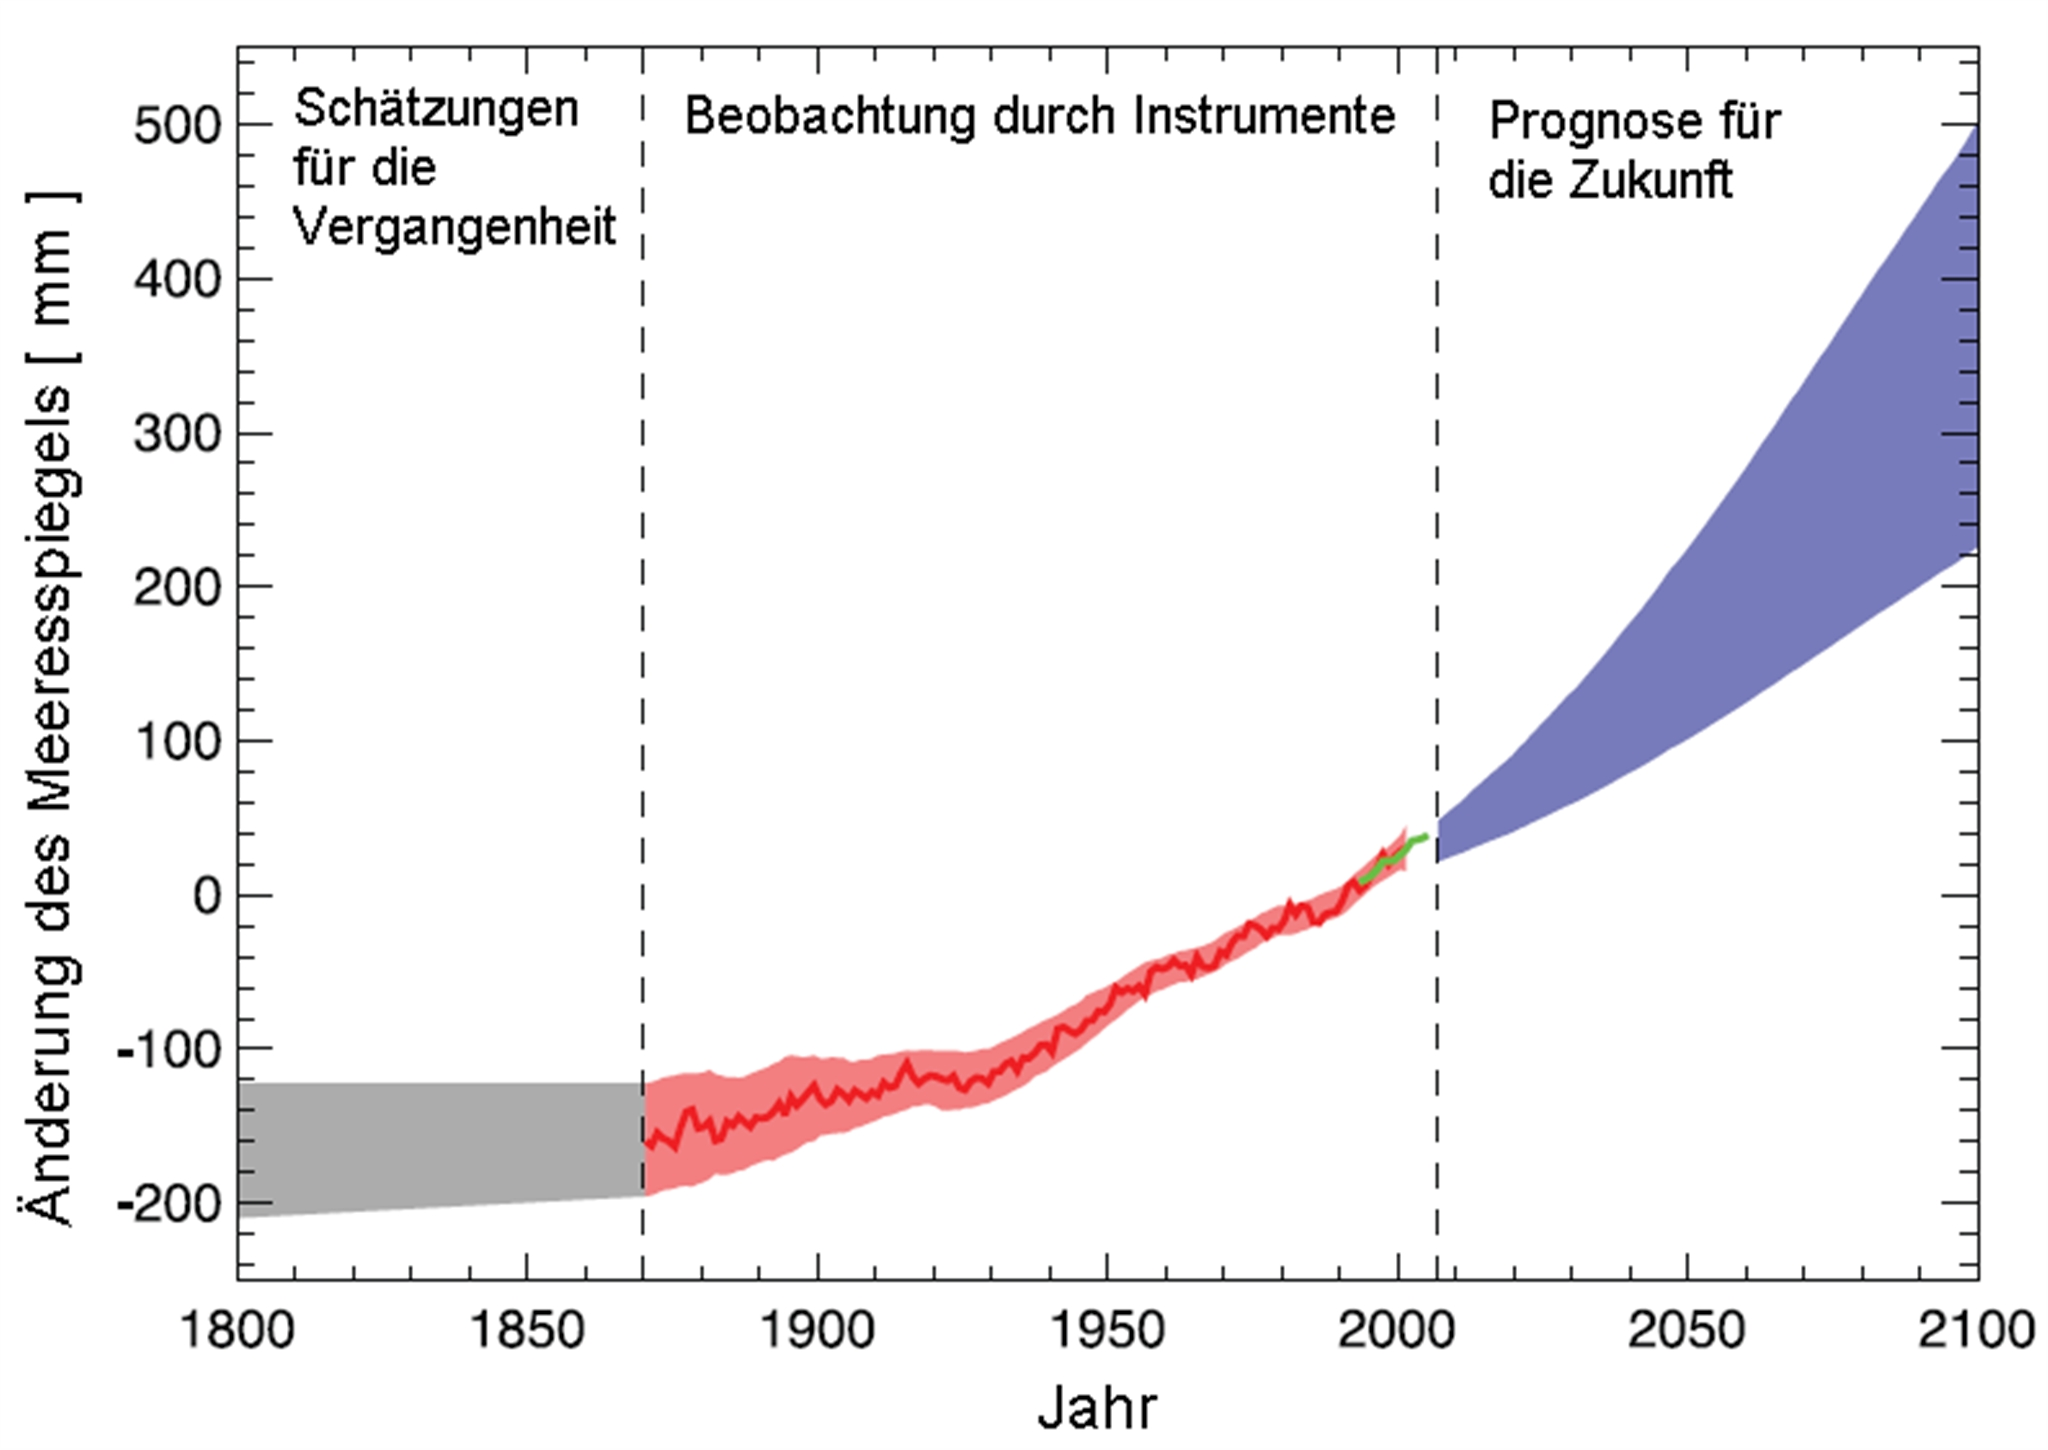
\includegraphics[width=1\textwidth]{images/anstieg.jpg}
\newline\newline


seit Anfang 20. Jahrhundert, 15
\newline
Da die Durchschnittstemperatur steigt, ,21. Jahrhundert = max 59 cm. 
+ Holland sinkt. (verkippen der Erdscholle) = um 10 cm bis zum 21. Jahrhundert
\newline
In Zukunft:  85 bis 130 cm pro Jahrhundert